\section{Descripción del prototipo} 
El prototipo actual busca definir el número de nodos y las características que estos deben tener para crear un ambiente de Big Data que nos permita realizar las pruebas a nuestro caso de estudio de manera satisfactoria pero que tampoco escape de las capacidades de computación con las que contamos.
\\
Por otro lado busca definir como serán agrupados los datos que conforman el caso de estudio en los nodos que se establezcan. Para poder conocer con ello la distribución de los datos y el peso en memoria física que se le dará a cada nodo.
\\
Se busca entonces encontrar características en común entre los datos que conforman el caso de estudio para de esta manera clasificarlos y facilitar su consulta al momento de aplicar algoritmos de minería de datos. 
\section{Análisis}
\subsection{Análisis de la red distribuida}\label{seccion1}
%necesidad
Se pretende establecer las características que tendrá el cluster que se aplicará a la red distribuida para poder con esto, generarlo. 
\\
A continuación, se presenta el análisis de los factores que se consideran importantes para dicho objetivo: 
\\
\begin{itemize}
\item Se definió que es necesario realizar una replica de los datos en los nodos ya que si la información original no esta disponible, en algún espacio en el tiempo se podrá utilizar la información de respaldo que se tiene de los mismos, con lo que se lograría que los datos sean mas persistentes.

\item Para poder almacenar 2 copias de la misma información la original  la replica, es necesario contar con al menos 2 nodos de datos y un nodo maestro. 

\item El nodo maestro no puede ser considerado nodo de datos ya que este cumple otra tarea, la cual es administrar y ordenar al resto de los nodos.

\item También se definió que para manejar datos de la dimensión de 21GB (tamaño de la base de datos del caso de estudio), nodos de datos de menos de 2GB de capacidad de RAM no son eficientes e incluso llegan a tener problemas con las configuraciones de memoria que se realizan mas adelante, por lo que se considera que los nodos de datos deberán trabajar con al menos 2GB de RAM.

\item Para poder comunicar el cluster dentro de una red local se utilizan 2 tecnologías Spark y Hadoop además de las dependencias de estas para funcionar como son SSH y Java. Por lo que es necesario considerar el espacio que ocupa la instalación de dichas tecnologías.

\end{itemize}
\subsection{Análisis de los datos} \label{datosagrupados}
La base de datos que se tiene planeado utilizar como caso de estudio tiene un total de 21GB de texto plano de información de productos que se venden en tiendas departamentales en la república mexicana. 
\\
Se trata de un archivo de datos de la PROFECO de uso libre el cual tiene los siguientes campos para cada producto.
\begin{lstlisting} 
	producto,presentacion,marca,categoria,catalogo,precio,fecharegistro,
	cadenacomercial,giro,nombrecomercial,direccion,estado,municipio,
	latitud,longitud
\end{lstlisting}
El archivo contiene toda clase de productos comerciales desde alimentos, electrónica, linea blanca, papelería, etc. 
Cada producto viene acompañado de la información de la tienda departamental que lo comercializa.
como ejemplo del contenido de dicho archivo se muestra los siguientes registros.
\begin{lstlisting} 

| crayones | caja 12 ceras. jumbo. c.b. 201423 | crayola 
| material escolar| utiles escolares | 27.5 | 2011-05-18 00:00:00 
| abastecedora lumen | papelerias | abastecedora lumen sucursal villa coapa 
| cannes no. 6 esq. canal de miramontes | distrito federal | tlalpan 
| 19.297 | -99.1254 |


| crayones | caja 12 ceras. tamano regular c.b. 201034| crayola | material escolar 
| utiles escolares | 13.9 | 2011-05-18 00:00:00 | abastecedora lumen | papelerias 
| abastecedora lumen sucursal villa coapa | cannes no. 6 esq. canal de miramontes 
| distrito federal | tlalpan | 19.297 | -99.1254 |


| galletas populares | paquete 170 gr. marias | gamesa | galletas pastas y 
harinas de trigo | mercados | 6.5 | 2011-01-10 00:00:00 | walmart 
| tienda de autoservicio | walmart | boulevard bernardo quintana no.4113 
esquina camino a sa| queretaro | santiago de queretaro  | 20.6162 | -100.398 |


| galletas populares | paquete 170 gr. marias | gamesa | galletas pastas y 
harinas de trigo | mercados | 6.6 | 2011-01-10 00:00:00 | farmacia guadalajara 
| tienda de autoservicio | farmacia guadalajara sucursal 326| ignacio picazo 
no.25 norte casi esquina allende ponien | tlaxcala | chiautempan | 19.3159 |-98.1945 |
\end{lstlisting}
Estos ejemplos que fueron tomados estratégicamente para ser analizados como se lista a continuación.
\begin{itemize}
	\item El archivo contiene información de varios productos que se venden en la misma tienda, conservando entonces la parte de datos referente a la tienda pero cambiando la parte del producto.
	\item El archivo contiene información del mismo producto vendido en varias tiendas departamentales en diferentes lugares, en esta caso, la información del producto es la misma mientras que la información de la tienda departamental cambia.
	\item El archivo contiene productos similares que se venden en la misma tienda o bien en otras tiendas que no son precisamente iguales pero que se pueden comparar entre ellos.
\end{itemize}
Usando el análisis formulado anteriormente se puede proponer diferentes alternativas de agrupación de los datos. Las que se consideraron se listan a continuación.
\begin{itemize}
	\item Precio del producto
	\item Categoría del producto
	\item Tienda departamental
	\item Zona Geográfica
	\item Estado de la república donde se encuentra el producto 
\end{itemize}

Por otro lado se determino que el sistema de almacenamiento de datos que se va a utilizar en la red distribuida, será Hadoop, y revisando su modo de operación y de manejo de archivos en su HDFS este no permite que la forma en la que se agrupan los datos sea definida por el usuario por lo que, los datos serán distribuidos siguiendo la técnica de Hadoop.

Es mas conveniente utilizar la forma en la que Hadoop distribuye los datos debido a que no es necesario controlar el acceso a los datos de manera manual indicando donde se encuentra cada uno de ellos, sino que Hadoop se encarga de esta tarea, además de ofrecer otros beneficios como la escalabilidad, la tolerancia a fallos , replicación en tiempo real, etc. 

A pesar de esto, el análisis realizado para determinar los modos de agrupamiento mas favorables no será desperdiciado pues este buscaba simplificar la operación de los algoritmos de minería de datos. y aunque no se aplique directamente sobre la distribución de los repositorios en los nodos, esta será aplicada al momento de ejecutar los algoritmos de minería de datos. 

\section{Diseño}
\subsection{Diseño de la red distribuida} \label{seccion2}
\subsubsection{Características de la red distribuida}
Las características que tiene la red distribuida se enlistan a continuación:
Se diseño una red distribuida que cuenta con 4 nodos en total.
\\ Un nodo que cumple la función de nodo maestro.
\\ Tres nodos que son utilizados como nodos de datos/replica.
\\ \\
Cada nodo usará la siguiente cantidad de memoria RAM:
\\ Nodo Maestro: 6.7 GB.
\\ Nodos Esclavos: 2 GB.
\\ 
\\ Se usa una conexión de red local para que los nodos puedan comunicarse.
\\ Se asigno una IP estática a cada nodo para evitar problemas con la asignación dinámica de IPs mediante DHCP.
\\ Cada nodo maestro y de datos/replica estará funcionando con base en un sistema operativo Ubuntu 16.04.
\\ 
\\ Se requiere que cada nodo de datos/replica cuente con 40 GB de almacenamiento en disco duro debido a que:
\\ Se almacenarán 21 GB de información, y 21 GB de réplica en los nodos de información y de réplica respectivamente entre los 3 nodos. 
\\ los programas que requieren tener en ejecución los nodos para funcionar correctamente, además de el sistema operativo los cuales ocupan 1.38GB de disco duro.
\\ El espacio reservado libre para que Hadoop haga sus cambios y modificaciones de archivos en tiempo real como este lo requiera.
\\ El espacio en disco libre que necesita el nodo para funcionar y seguir procesando datos.
\\
Sólo los nodos de datos/replica almacenan y procesan información 
\\ El nodo maestro administra y ordena.
Cada nodo funciona con Apache Spark 2.7 y Hadoop 3.1.1.
\subsubsection{Red distribuida en la arquitectura del sistema}
El diseño de la arquitectura del sistema y la red distribuida se muestran en la figura \ref{fig:red}.
\\ 
Como se puede observar en la arquitectura se tiene un nodo maestro y tres nodos de datos/replica conectados a través de Hadoop.
\\
Se explicará como se busca que estos trabajen en conjunto una vez que todos los prototipos se encuentren terminados y como el diseño existente hasta este momento estará afectando dicho comportamiento.
\\
El nodo maestro será el nodo donde el usuario experto instalará el ambiente para hacer uso de big data y configura sus nodos, una vez que la instalación sea exitosa podrá ingresar sus datos, seleccionar los algoritmos que desea aplicar a los mismos y visualizará los resultados.
\\
Mientras el usuario solicita operaciones directamente desde el nodo maestro los nodos de datos o replica se encontrarán accediendo a los datos que se encuentran alojados en cada
uno de ellos y ejecutando las operaciones que se les soliciten sobre los mismos las solicitudes antes mencionadas serán hechas en su totalidad por el nodo maestro. 
\\
Posteriormente los resultados parciales obtenidos en cada uno de los nodos serán devueltos al nodo maestro para que este pueda generar el resultado final utilizando los resultados parciales de cada uno de los nodos y mostrarlo al usuario experto.

\begin{figure}[!htbp]
	\hypertarget{fig:red}{\hspace{1pt}}
	\begin{center}
		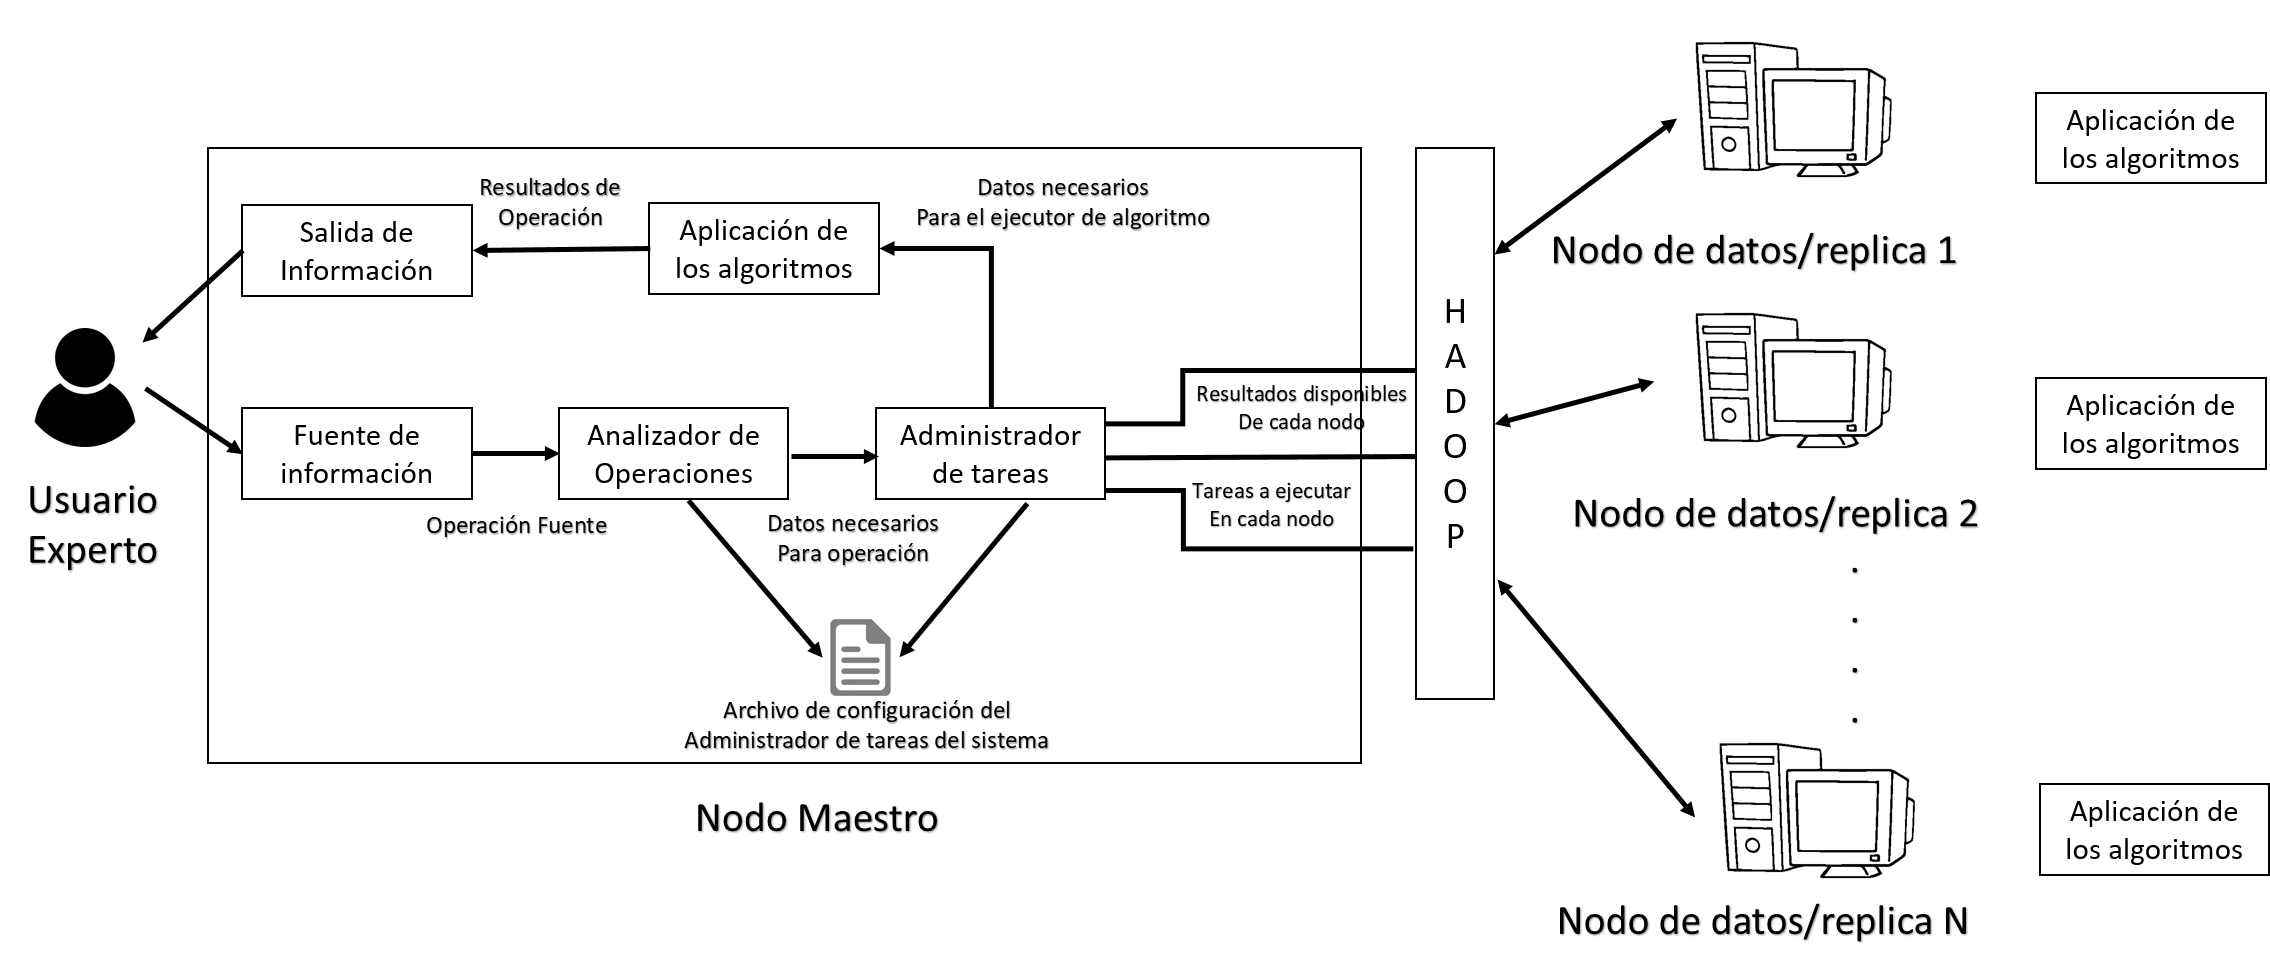
\includegraphics[width=.7\textwidth]{capitulo3/images/im1.png}
		\caption{Arquitectura del sistema}
		\label{fig:red}
	\end{center}
\end{figure}

\subsection{Diseño de propuesta de agrupación de acuerdo a los nodos definidos en la red distribuida}

Al usar una tecnología como Hadoop, este mismo es capaz de distribuir los datos sin que se diseñe una
propuesta de agrupación por parte del programador sino que, Hadoop establece la propia.
\\
Hadoop dentro de su arquitectura cuenta con un bloque conocido como HDFS en cual es un sistema de archivos distribuido y tolerante a fallos. Funciona sobre el conjunto de los nodos
de un cluster de Hadoop, balanceando la carga de archivos entre las máquinas del cluster,
de forma equitativa. Gracias a su naturaleza distribuida, proporciona alta disponibilidad y
altas prestaciones que le permiten ser capaz de manejar archivos de gran tamaño.
\\
Para realizar esta tarea es necesario proporcionarle el archivo de datos completo a HDFS e indicarle el número de copias que se harán de los datos,  el archivo proporcionado será segmentado en bloques de 128 MB por parte de Hadoop como se muestra en la figura \ref{fig:red2}.
\begin{figure}[!htbp]
	\hypertarget{fig:red2}{\hspace{1pt}}
	\begin{center}
		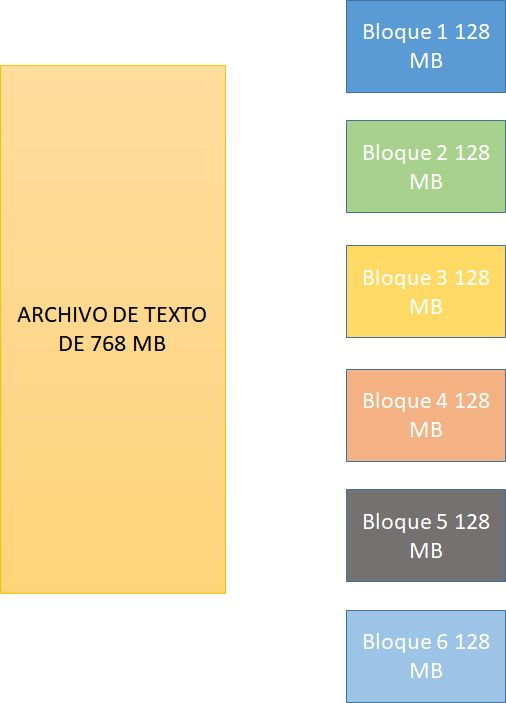
\includegraphics[width=.4\textwidth]{capitulo3/images/im2.png}
		\caption{Generación de bloques de un archivo}
		\label{fig:red2}
	\end{center}
\end{figure}
\newpage
El sistema de Hadoop ingresará cada bloque considerando este bloque como bloque de
datos en algún nodo y para las réplicas ingresara nuevamente el bloque considerando este
bloque como bloque de replica 1, bloque de réplica 2 , bloque de réplica 3 y continua de la
misma forma para la cantidad de bloques de réplica que se hayan indicado. Para cada una
de las réplicas es indispensable que no sean asignadas en el mismo nodo que el bloque de
datos o alguna otra réplica. No tiene sentido realizar más o igual número de réplicas que de
nodos, debido a que las réplicas se realizan para garantizar el acceso a los bloques en todo
momento, y si el bloque es accesible en un nodo y la réplica se encuentra en el mismo
nunca sería utilizada.
\\
Para ejemplificar la explicación anterior se mostrará la distribución que haría Hadoop para un sistema de 3 nodos con una réplica en
la imagen \ref{fig:red3}.
\newpage
\begin{figure}[!htbp]
	\hypertarget{fig:red3}{\hspace{1pt}}
	\begin{center}
		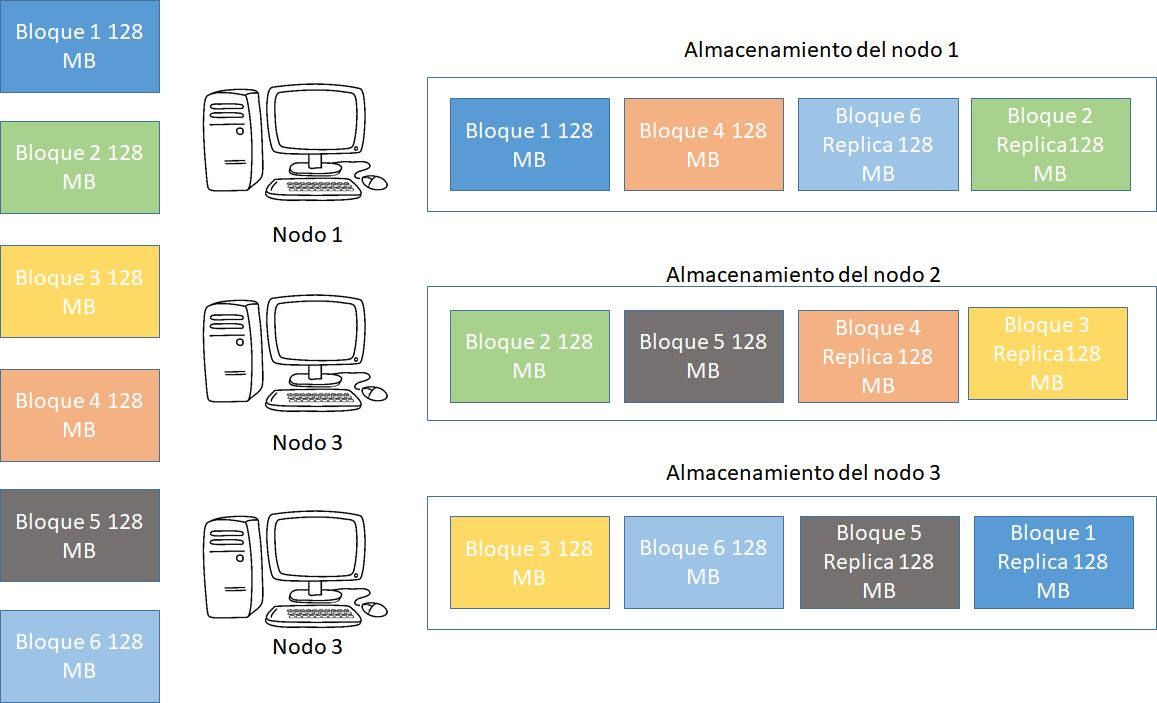
\includegraphics[width=.7\textwidth]{capitulo3/images/im3.png}
		\caption{Generación de bloques de un archivo}
		\label{fig:red3}
	\end{center}
\end{figure}
Por lo que podemos ver que en caso de que alguno de los nodos deje de responder en los
otros 2 nodos tenemos acceso a todos los datos, ya sea en el bloque de datos o en el
bloque de réplica, hecho que no ocurriría en caso de que 2 nodos dejen de responder, el
cual se solventa realizando 2 réplicas de los datos.
\\
En tiempo de ejecución, para realizar su trabajo Hadoop siempre toma en cuenta primeramente los bloques de datos
y en caso de no encontrarlos procede a hacer uso de las réplicas generadas de los mismos.
\\
En el servidor maestro se guarda una información conocida como NameNode que permite
conocer dónde se encuentran cada uno de los bloques y sus réplicas, lo que facilita sean encontradas dentro del cluster.
\\
Con lo que podemos concluir que si bien no diseñamos la propuesta de agrupación de los datos comprendemos cómo es que esta funciona.
\section{Desarrollo}\label{seccion3}
Para que la red distribuida se encuentre en funcionamiento se siguió el Manual de Instalación de Luminus 
en sus secciones 
\begin{verbatim}
1 Instalación de Apache Spark en el nodo
	1.1. Instalación de la paquetería de java 
	1.2. Instalación de la paquetería de SSH	
	 1.2.1. Configuración
	 1.2.2. Conexión
	1.3. Instalación de Spark
     1.3.1. Configuración maestro

2. Instalación de Apache Spark en los nodos de datos
	2.1. Instalación de la paquetería de java en los nodos de datos
	2.2. Instalación de la paquetería de SSH en los nodos de datos
	2.3. Instalación de Spark en los nodos de datos
     2.3.1. Configuración 
3. Puesta en funcionamiento
	3.1. Configuraciones para poner en funcionamiento Apache Spark en la red distribuida
\end{verbatim}
Las cuales nos permitirán instalar Apache Spark para permitir la conexión entre los nodos de datos/replica y el maestro haciendo uso de una red de internet local en la que se encuentren conectados todos los nodos.
\\
Además de contener todas las configuraciones necesarias para tal objetivo.  
\section{Pruebas}\label{seccion4}
Para verificar que la instalación y configuración que se realizo al servidor Apache Spark es correcta será necesario aplicar un algoritmo de prueba. 
\\
Un algoritmo de prueba muy común es sparkPi el cual calcula el valor del número pi utilizando todos los nodos de la red distribuida. 
\\
Esto nos permitirá comprobar que existe conectividad dentro de la red y que se pueden realizar calculos con ella.
\\
El comando a ejecutar es el siguiente 
\begin{lstlisting} 
MASTER=spark://[IP del nodo maestro]:7077 run-example SparkPi
\end{lstlisting}
como se puede apreciar en la siguiente imagen \\
\begin{figure}[!htbp]
	\hypertarget{fig:red4}{\hspace{1pt}}
	\begin{center}
		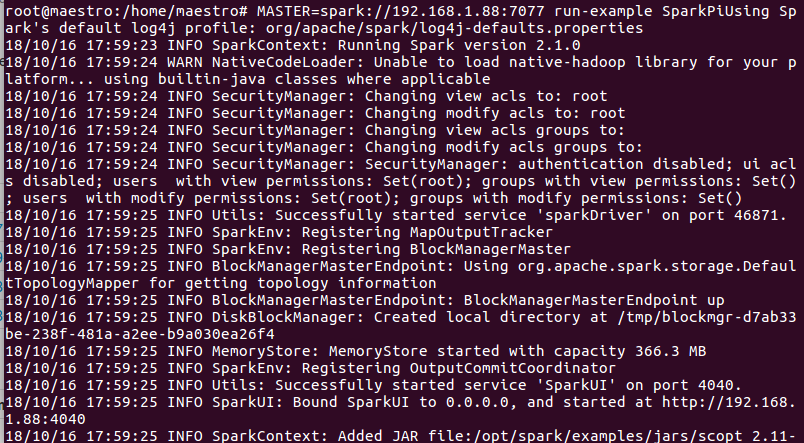
\includegraphics[width=.7\textwidth]{capitulo3/images/im9.png}
		\caption{Ejecución de algoritmo SparkPi}
		\label{fig:red4}
	\end{center}
\end{figure}
\\ cuando este termine podremos ver el resultado del valor de PI en la consola \\
\begin{figure}[!htbp]
	\hypertarget{fig:red5}{\hspace{1pt}}
	\begin{center}
		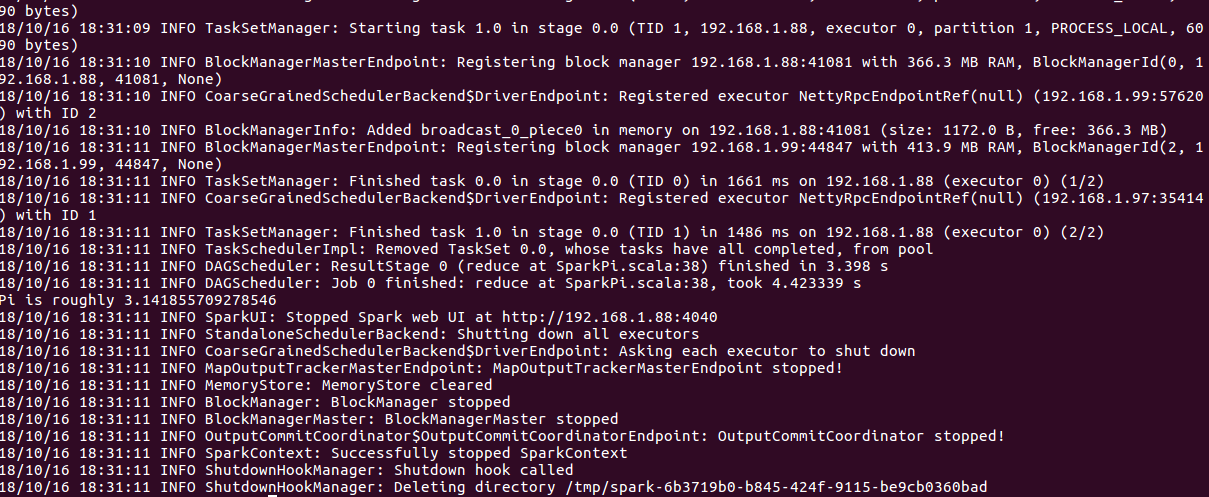
\includegraphics[width=.7\textwidth]{capitulo3/images/im12.png}
		\caption{Valor de PI}
		\label{fig:red5}
	\end{center}
\end{figure}
\\ cabe destacar que debido a que el valor es calculado en tiempo real con los recursos que se tiene en el cluster el valor puede variar cada ejecución pero será muy aproximado al valor real del número.
\\
Ahora, si accedemos a la interfaz web de Spark podremos ver que un trabajo ha sido completado dentro del cluster, antes de esta ejecución no se mostraba nada dentro de esta sección. \\
\begin{figure}[!htbp]
	\hypertarget{fig:red6}{\hspace{1pt}}
	\begin{center}
		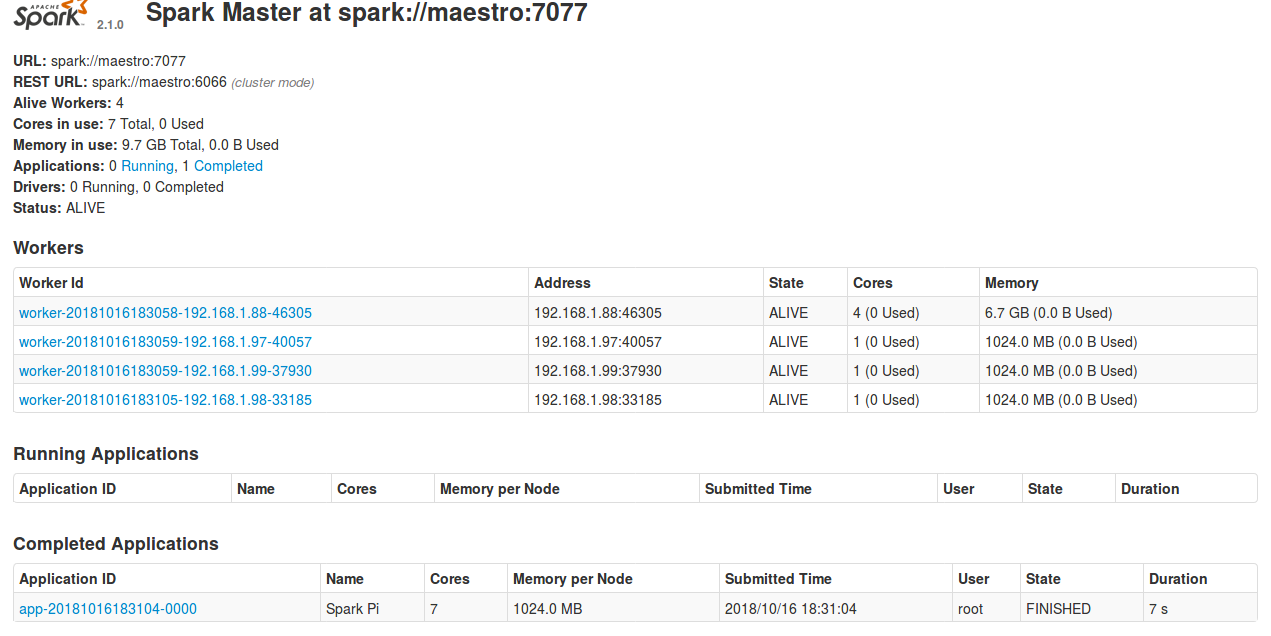
\includegraphics[width=.7\textwidth]{capitulo3/images/im6.png}
		\caption{Aplicación completada en Apache Spark}
		\label{fig:red6}
	\end{center}
\end{figure}
\\ En caso de entrar a los detalles de la misma podremos observar que todos los trabajadores participaron en dicha aplicación y que se encuentran en el estado muerto debido a que la aplicación a finalizado su ejecución. 
\\ así como también podemos visualizar los archivos de registro que generaron durante la ejecución de esta aplicación, entre otros detalles.
\begin{figure}[!htbp]
	\hypertarget{fig:red7}{\hspace{1pt}}
	\begin{center}
		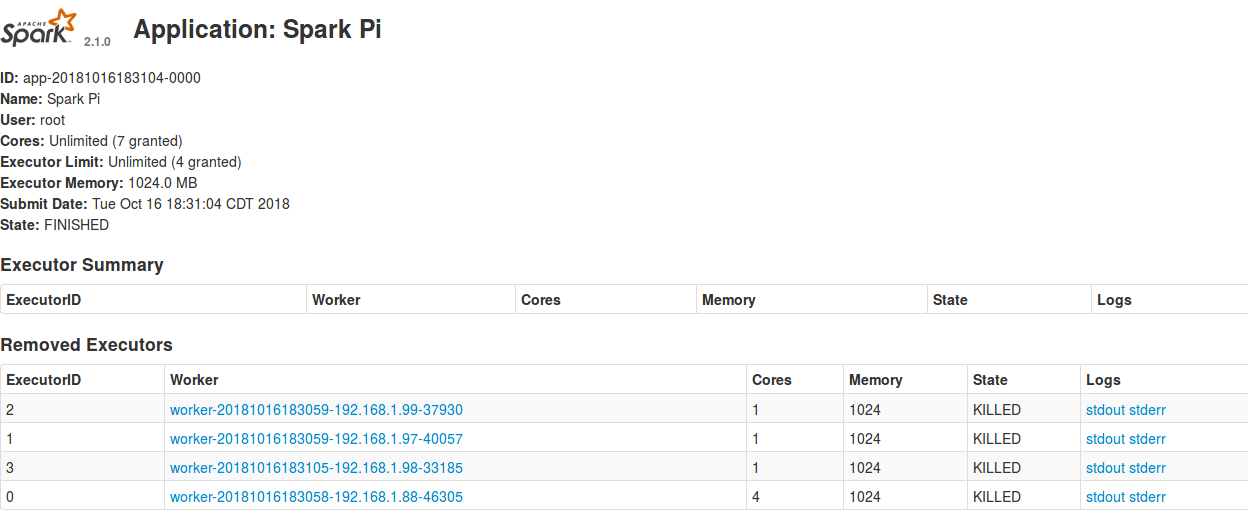
\includegraphics[width=.7\textwidth]{capitulo3/images/im10.png}
		\caption{Detalles de la ejecución de la aplicación Spark Pi}
		\label{fig:red7}
	\end{center}
\end{figure}
otro punto importante es que también se puede consultar para cada uno de los nodos su participación en la ejecución de esta aplicación como se muestra en la figura \ref{fig:red8} para el caso del nodo maestro
\newpage
\begin{figure}[!htbp]
	\hypertarget{fig:red8}{\hspace{1pt}}
	\begin{center}
		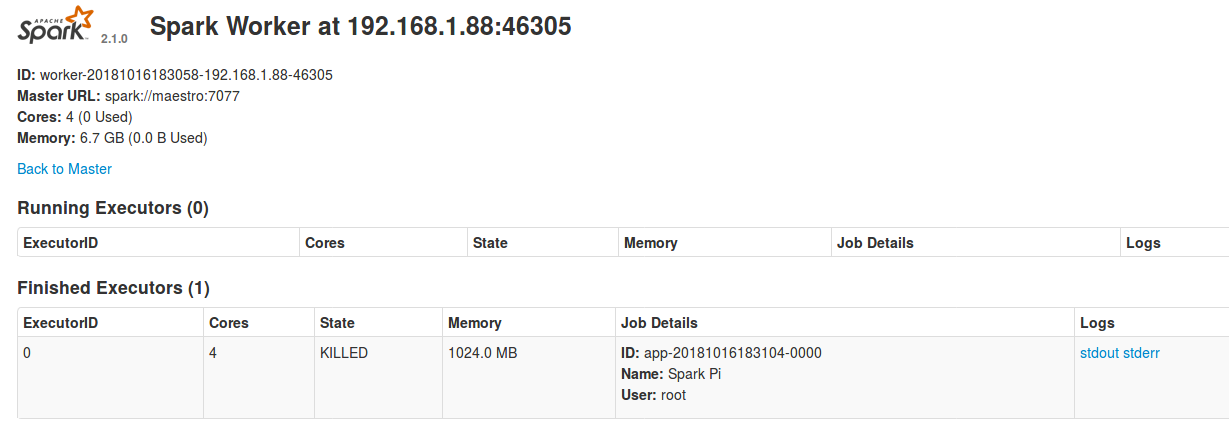
\includegraphics[width=.7\textwidth]{capitulo3/images/im11.png}
		\caption{Detalles de la ejecución de la aplicación Spark Pi en un nodo}
		\label{fig:red8}
	\end{center}
\end{figure}

Con lo que podemos concluir:
\begin{itemize}
	\item El cluster funciona correctamente
	\item Existe comunicación entre los nodos
	\item Los nodos de datos/replica son capaces de identificar al nodo maestro y recibir instrucciones de el
	\item El nodo maestro es capaz de comunicar trabajos a los nodos de datos/replica y de interpretar los resultados de sus trabajos de manera satisfactoria
\end{itemize}
Por lo tanto, el prototipo uno concluye de manera exitosa

